\documentclass[../../thesis.tex]{subfiles}
\graphicspath{{\subfix{diagrams/}}}

\begin{document}
The goal of the work is to explore if zk-rollups can be used to aggregate Uniswap trades in an effective manner. The prototype is able to aggregate trades for a single trading pair, Ether and an ERC-20 token of choice. First, we'll look at the systems design to understand how the different entities work together.


The system consists of two main entites that are required for it to function. The first entity to look at, is the on-chain entity, we call zkSwap. zkSwap is a smart-contract deployed on the Ethereum blockchain and has three main jobs, processing deposits and withdraws, aswell as verifying batched trades. It holds users funds and exposes the on-chain functionality, namely deposits and withdrawls, to the user. 

The second entity to look at is the aggregator. The aggregator consists numerous systems, both off-chain and on-chain, and is mainly tasked with receiving trade orders, aggregating and executing them, and then verifying them with the zkSwap contract. The aggregator stores a merkle-tree of users balances and keeps it in sync by listening for event emitted by the zkSwap contract.

\begin{figure}[h]
    \centerline{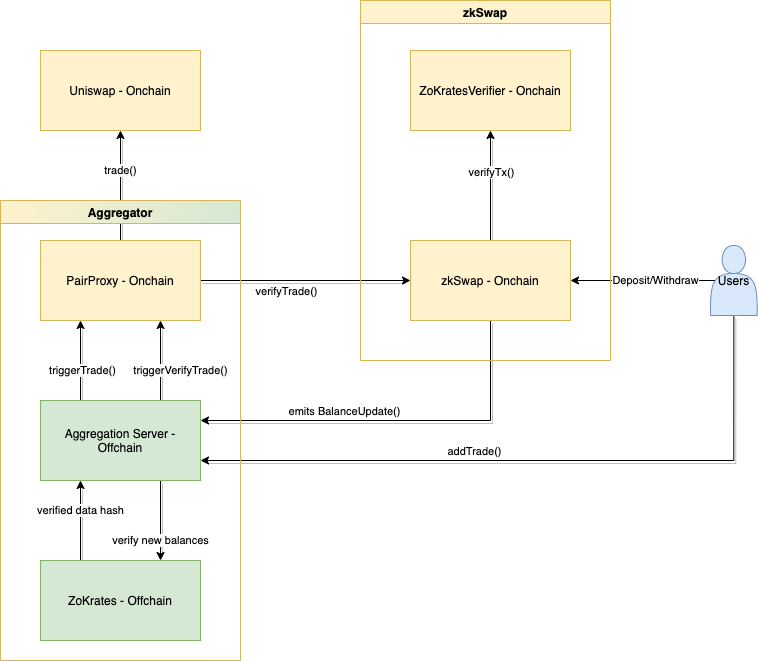
\includegraphics[totalheight=8cm]{diagrams/architecture.png}}
    \caption{High level architecture of the system}
    \label{fig:architecture}
\end{figure}

\subsection{Design}
In this section we will explore the design of the system, looking at the different functionalities and dependencies to understand the core mechanics of how the different entities interact with each other. 

The two main entities of this system are the zkSwap smart contract and the aggragator. 


\subsubsection{zkSwap Smart-contract}
The zkSwap contract, is the core entity the user interacts with. Its a smart-contract, that from the users perspective, is mainly used for depositing and withdrawing funds in out system and keeping track of user balances.

\paragraph{Deposits}
To use the system a user first has to deposit funds into the smart-contract. The funds need to be sent as a normal on-chain transaction to the smart-contract, where they will be stored, while the balance is then represented in layer-2. To deposit funds, a user calls the deposit function in the zkSwap smart-contract and adds the funds to be deposited to the transaction. When the funds have been received, an event is emited informing the aggregator about the new deposit. At the same time, the user signs the deposit data, and sends it to the aggregator as a message. The aggregator aggregates a number of deposits, verifies the correctness in the zkSwap smart-contract, at which point they will show up as balance for the user.

\paragraph{Withdraws}
When withdrawing funds, the user needs to decide between an aggregated withdraw, similar to the deposit, or an instant on-chain withdraw. The aggregated withdraw works just like the deposit, only difference being the a withdraw amount is specified instead of sending funds. After the aggregation is complete, the user will receive the funds as an on-chain transaction. A user can also withdraw funds by using the instant withdraw feature. While it costs significantly more gas to withdraw funds with this function, it can be used without the aggregator being online. The protects the user from not being able to withdraw its funds in case the aggregator is offline or has turned malicious. 

\paragraph{Verification of Aggregated Trades}
The last main functionality of the zkSwap contract is the verification of aggregated trades. Once the aggregator has completed the aggregation batch, it send the new balances along with a zkSNARK proof and the traded funds to the zkSwap contract. If the proof is valid and the correct amount of funds have been sent to the zkSwap contract, the new balances are emitted, finanlizing the state. The aggregator is now refunded, receiving the funds it spent when executing the aggregated trade on Uniswap.

\subsubsection{Aggregator}
As the name implies, the aggregators job is aggregating deposits, withdraws and trades. The aggregator relies on a number of different systems to function, in the section we look at it from a functional perspective, explaining the core functionalities and what systems is relied on. This will be explained in the implementation section in more detail.

\paragraph{Deposits and Withdraws}
When a user deposits or withdraws funds, choosing the aggregated type, the user sends a signature of the deposit/withdraw operation to the aggregator. The aggregator receives theses messages, collecting them as the next aggregation batch. Once a number of messages have been received, the new balances are caluculated and passed to the corresponding ZoKrates program, where the correctness of the balances and signature is checked. If this is successful, a zkSNARK proof object is created. The aggregator now send the proof, along with the new balances to the zkSwap smart-contract. If the proof is valid, the new balances are emitted by the zkSwap contract. Each withdraw will now be credited by sending the requested funds to the users. 

\paragraph{Aggregating Trades}
A user can make a trade by sending a message to the aggregator. Similarly to deposits and withdraws, the aggregator collects messages as the next aggregation batch. All received trade messages are now aggregated and offset internally, resulting in the 'net-trade' that must be executed to honor all trades of the batch. The 'net-trade' is then sent to the 'PairProxy' smart-contract as a on-chain transaction, which in turn will execute it on Uniswap. The details and reasoning of this contract will be explained in the implementation section. Once the trade is executed, the new balances are calculated and the correctness ensured by using the corresponding ZoKrates program. The resulting proof and the new balances are sent to the PairProxy smart-contract. The previously purchased funds are now added to the transaction, forwarding it to the zkSwap smart-contract. The proof is verified, the new balances emitted, and the aggregator is refunded the amount paid in the 'net-trade'. 

\paragraph{Storing Balances and Generating Proofs}
The aggregator keeps track of the balances by listening to events emitted by the zkSwap smart-contract. When an event is received, the aggregator updates the balances locally. Since events stay on-chain, the balances can always be reconstructed by querying them sequentially. Storing all balances enables the aggregator to generate proofs that are needed thoughout the system.

\subsection{Implementation}

\subsection{zkSwap Contract}
The zkSwap contract, is the core entity the user interacts with. Its a smart-contract, that from the users perspective, is mainly used for depositing and withdrawing funds in out system. 

\subsubsection{Storing and Updating Balances} \label{balances}
Two main factors are dictating the way balances are stored in the system. It is important to understand the core technique used to store and update balances before we look at the different functions that trigger them. We want to make balance updates as cheap as possible, while not relying on any external data availability. Essentially, this means that we need to store the balances on-chain. Storing data on-chain is typically very expensive. It is important to make a distinction between storing data in a smart-contracts runtime \todo{is runtime the correct word?} and storing data in the event log. Both methods of storage are on-chain, using the event log is significantly cheaper though. A disadvantage of using the event log however, is the fact that it can't be accessed from a smart-contract runtime, but must be queried by a client. This solves the external data availablity problem. We can store balances cheaply by emitting the `BalanceUpdate' event, without relying on other systems to stay online. A client can query the event log, gather the required data and pass it as parameters to the transaction. However, we now need a mechansism to ensure, the user is passing correct data. 

\paragraph{Merkle Trees}
We can achive this, be using a merkle tree \cite{szydlo2004merkle}. Merkle trees are a suitable data structure, as the merkle root represents the entire tree state in a highly compressed form, while proving a leafs inclusion in the tree can be done with O(log n). This is ideal for our use-case. Every balance is stored as a leaf in a merkle tree, running in layer-2. The merkle tree is built and kept in sync by subscribing to the ‘BalanceUpdate’ event emitted by our smart-contract. A client can query balances from this  tree, receiving the valid merkle path along with the balance object. The correctness of that data can be proven by recreating the merkle root, which is stored and updated in the zkSwap smart-contract. Since all changes in balance are committed by emitting the `BalanceUpdate' event, it must be ensured that merkle root is changed according to the updated balance. It is important to understand, that the only way balances can be updated is with the `BalanceUpdate' event.


\subsubsection{Aggregating Balance Updates}
Updating a users balance is at the core of this system. Deposits results in a balance update, as do trades and withdraws. Before looking at these in detail, it is important to understand how balance updates can be aggregated, reducing the transaction costs for these operations. Since balances are stored in a merkle tree, we can ensure the correctness of a balance by running an inclusion proof. However, running this in a smart-contract is expensive, as a lot of hashing is required. To reduce this cost, we can ensure the correctness by running this in a ZoKrates progam. If the ZoKrates program exits successfully, a zkSNARK proof is generated, which can be used to verify our execution on-chain.   

 
\paragraph{Merkle Inclusion Proofs}
In order to ensure the correctness of balance updates, we first need to verify the inclusion of the balances involed in the merkle tree. Doing this one by one is simple. Every balance provides its merkle path which can be hashed with the leaf. If the merkle root matches the current merkle root stored in the zkSwap smart-contract, we can be assured the provided balance leaf is correct. At the same time, this enables us to reuse the merkle path for updating the balance leaf. We can simply change the balance leafs values after passing the inclusion proof, rehash with the merkle path, and the result is the correct root for the updated balance leaf.

\paragraph{Chaining Inclusion Proofs} \label{chain_inclusion}
When dealing with multiple balance leafs, the inclusion proof can be done the same way. Every balance leaf provides its merkle path, the resulting hash should be the same for each leaf. Things become more difficult when updating the balance leafs. Updating the first leaf in the batch now invalidates the merkle path of all following leafs. In order for this to work, the merkle paths for each balance must be created sequetually. This can be solved by sorting the leafs before hand, and generating each merkle path based on the changes of the previous balance. The new root of the first balance is the old root of the next balance. This can be chained to an infite length and results in a constant number of hashes required for each balance update. The last hash to be computed is the new merkle root, representing all balance updates.

(Add Algo here)

\paragraph{Authorizing Balance Updates}
We still need to ensure the user has authorized this balance update though. As balance updates are emitted as an event, anyone can access them and compute valid merkle paths for any balance. This would, for example, allow any user to withdraw any balance. To ensure a user is authorized to update a balance, we need ensure the user controlls the private key belonging to the balances user address. This can be achived by requesting a signature from the user. However, it must be remembered, that this signature must also be verifiable in our ZoKrates programm, which is unable to utilize the secp256k1 curve, used for signing Ethereum transaction, efficiently \cite{deml_2019}. For that reason the BN128 curve is used in combination with the EdDSA signature scheme, which can be more efficiently run in a ZoKrates program. The user submits a signature containing the current merkle root and the update message. This ensures two things. It proves that the user has access to the addresses private key, which authorizes the trade order. By signing the current merkle root, we make sure, that the signature can't by reused in a replay attack. For instance, the aggregator could decide to store these signatures secretly, and reuse them without the users consent if this was omitted. It is important to note, that different programs are used for deposits/withdraws and trade aggregation. As already mentioned above, these programs have a number of checks that ensure the update message is valid. These will be explained in the respective sections. 

\paragraph{Executing and Reducing On-chain Verification Costs} \label{exec_and_reduce}
All of these checks are performed as a ZoKrates program. If no checks fail, the proof can now be generated.  We have now successfully verified the new balances, and we could use these values to generate the proof, which will then be used to verify everything on-chain. When verifying the ZoKrates program on-chain, each output of the program is part of the proof object, adding an iteration to the proving logic. The amount of outputs the ZoKrates program has, influences the verifications costs. We can reduce this cost by returning a hash of the resulting data, thereby reducing the amount of outputs. Since the aggregator computed the balances in the first place, and the ZoKrates program only verified it, it can pass that data as part of the verify transaction, but excluded from the ZoKrates proof object. By hashing the data with the SHA256 hashing algorithm in the zkSwap smart contract, we can ensure that data correctness by comparing it to the hash that is part of the proof object. As a result, the ZoKrates program only returns this hash as an output value. 

\subsubsection{Deposit}
When using the system, a user first has to deposit funds. Since the entire idea of zk-rollup is to move funds to layer-2, the deposit function can be seen as a bridge that connects the mainnet and layer-2. When a user makes a deposit, the funds are represented as a balance object in layer-2, which in turn give custody to these funds. When moving funds in layer-2, we don't actually move the funds residing in the smart-contract, but update the balance objects to represent the movement and verify that movement for correctness with a zkSNARK proof\todo{Maybe remove this?}. Since a balance object gives a user custody of represented funds, it can always be redeemed, moving from layer-2 back to mainnet.  

\paragraph{Movement of Funds}
To move funds to layer-2, a user first needs to send the funds to the zkSwap smart-contract. This is done by calling the deposit function in the zkSwap smart-contract and attaching the funds to the transaction. The deposit function now emits a `Deposit' event, containing the type of fund (Ether or ERC20), the amount and the address of the user making the deposit. This event notifies the aggregator of the deposit and ensures the user has actually deposited a certain amount of funds. It is important to note, that the deposit not finalized yet. 

\paragraph{Aggregating Deposits}
After the funds have been sent to the smart-contract, the user creates a signature containing the type of fund, the amount the users address and the current merkle root. This signature is sent to the aggregator as an HTTP request. The aggregator checks the signature of each incoming request and makes sure a matching `Deposit' event has been emitted. This ensures the user has actually sent funds to the smart-contract. After a number of deposits have been received, the aggregation is started. The aggregator now generates a `BalanceMovementObject' for each deposit, containing the old balance, the new balance, the merkle path and the signature. This is passed to the `ProcessBalanceMovement' ZoKrates program, along with the current merkle root. As explained in S. \ref{chain_inclusion}, the inclusion proof is now performed on the old balance. If the old balance is correct, the signature is checked, along with the change in balance. The signed amount should equal the added amount in the new balance, the nonce must be incremented and the address the same. If these checks pass for all `BalanceMovementObjects', we hash all new balances, as explained in S. \ref{exec_and_reduce}, along with the old merkle root and the new merkle root, to reduce the on chain verification costs.

\paragraph{Verifying Deposits On-chain}
Once the ZoKrates program has run successfully, the proof can be generated, which is used for verification in the zkSwap smart-contract. The aggregator sends the proof, along with the new balances and the old and new merkle root. As a first step, the balances and roots are hashed, and the result of the hash compared to the output field in the ZoKrates proof object. If these hashes match, we can be assured, the the aggregator has attatched the same data that has been checked by the ZoKrates program. Next, we check if the old root, matches the current root stored in the zkSwap smart-contract. This ensures that a generated proof can't be reused in replay attacks. As a last check, the ZoKrates proof object is checked with the verifier smart-contract deployed for this purpose. If this is also successful, we have proven, that the aggregator has proccessed the deposits correctly. We now iterativly emit the new balances with the `BalanceUpdate' event, and update the merkle root in the smart-contract. The deposits have now been processed aqnd show up as balance in the users account. 

\subsubsection{Aggregated Withdraws} \label{with}
The aggregated withdraws largly follow the logic of the deposits, so only the core differences will be explained here. Instead of sending funds to the zkSwap smart-contract, we are requesting them. Since the user already has a balance in the system, we don't need to notify the aggregator about the amount a user wants to withdraw, which in turn means we don't need an on-chain transaction to trigger the withdraw. A user creates a signature of its address, the current merkle root, type of funds and the amount to be withdrawn, and sends it to the aggregator as an HTTP request. Once the aggregation starts, the aggregator checks the users signature, and ensures that the users balance covers the withdraw. Just like with deposits, a `BalanceMovementObject' is created, the type being set to withdraw. The withdraws are verified with the deposits together, which reduces verification costs. The `ProcessBalanceMovement' checks signature, the balances and if the balances follow the withdraw request. On top of hashing the new balances, a withdraw object is also hashed, containing the type of funds and the amount. When verifying withdraws, along with the deposits, the withdraw objects will be used to send the funds from the smart-contract to the users. The new balances are emitted and the root updated. 

\subsubsection{Instant Withdraws}
A user also has the option to withdraw instantly, without being dependant on the aggregator. This ensures a user can always withdraw funds, even when the aggregator is failing or is offline. Instead of sending the withdraw request to the aggregator, the withdraw is processed completly on-chain. The user attaches its balance object, along with the corresponding merkle path and the withdraw amount and type to the transaction. As a first step, the merkle inclusion proof is performed. The balance object is hashed, sequeutually with the merkle path. The resulting hash now equals the the merkle root stored in the zkSwap smart-contract if the correct balance and merkle path have been submitted. It is checked if the balance can cover the withdraw, if thats the case the nonce is incremented, the new balance is calculated, and the new balance object hashed again. The new root is now computed by hashing with the merkle path, and updated in the smart-contract. The funds are now sent to the user and the new balance is emitted. It must be reiterated, that this is done completly on-chain and doesn't require the aggregator to be online. However, the gas costs of this transaction are significant, as hashing with the MiMC hashing algorithm is expensive in a smart-contract.

\paragraph{Authorizing Instant Withdraws}
This however, is an incomplete explaination, as we're not checking if a user is permitted to deposit or withdraw funds. As balance objects are emitted as an event, anyone can access them and compute valid merkle paths for any balance. This would allow any user to withdraw any balance. To ensure a user is permitted to update a balance object, we need ensure the user controlls the private key belonging to the balance objects user address. Fortunetly, we can ensure this by accessing the sender in transaction object. The Ethereum blockchain ensures a user is allowed to make a transaction by requiering the transaction to be signed with the private key of the senders address. If that signature is valid, it is proven that the user has access to the addresses private key and the transaction can be executed. Because of this, the transactions object sender can be trusted to be in controll of the corresponding private key. Instead of passing the users address as part of the balance object, the smart-contract uses the sender of the transaction object. This suffices as a security check.

% \paragraph{Merkle Inclusion Proofs}
% As described in S. \ref{balances} balance updates are secured by merkle inclusion proofs in the smart-contract. When depositing the user needs to provide a valid merkle path to its balance object, and the balance object itself. The balance object consists of four fields that are needed to represent the balance: ethAmount, tokenAmount, nonce and userAddress. As a first step, the balance object is hashed with the sha256 algorithm, the result being the leaf in the merkle tree. The leaf is now hashed with the merkle path, according to the standart merkle root hashing algorithm. If the resulting hash equals the stored balance root in the contract, we have proven, that the passed balance object is correct. We now add the value of the transaction object, which is the deposit amount sent with the transaction, to the ethAmount, increment the nonce and hash the new balance. Since the balance object has the same position in the tree, the same merkle path is also valid for the new balance. The new leaf is hashed with the merkle path, and the resulting hash is set as the new balance root. As a last step we emit the `BalanceUpdate' event, containing the new balance object, matching the balances with the newly set root. 

% Withdraws largely follow the same logic, there are small differences though. As we're requesting funds, instead of sending them, we pass a withdrawAmount as an additional parameter to the function call. We then check if the withdrawAmount <= ethAmount to make sure the withdraw is covered by the users balance. The inclusion proofs are the same, we then subtract the withdrawAmount from the balance, and update the balance root. As a last step we emit the `BalanceUpdate' event with the new balance object, and send requested funds to the user as an on-chain transaction.



% It must also be noted, that ERC-20 deposits and withdraws behave a bit differently. As every ERC-20 token has its own smart-contract, representing a users balance as a mapping, we need to transfer the assets in that contract. This requires different functions to handle ERC-20 deposits and withdraws, however implementing this is trivial and not worth explaining in the context of this work. 

\begin{figure}[h]
    \centerline{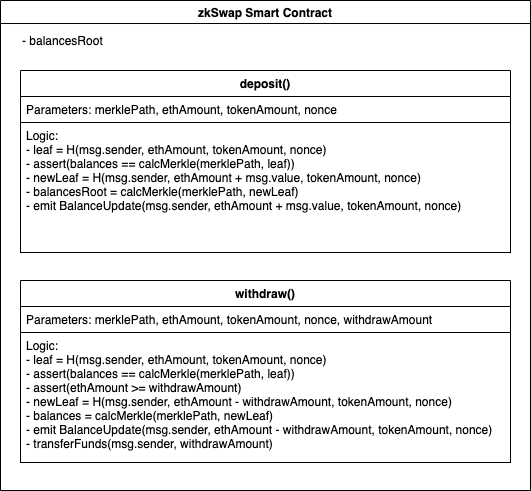
\includegraphics[totalheight=8cm]{diagrams/deposit.png}}
    \caption{Pseudocode of the deposit and withdraw steps}
    \label{fig:dep_with}
\end{figure}


\subsubsection{Batch Verification of Trades}
It is recommended to read S. \ref{aggregator} first, as is covers the previous steps of a trade aggregation life-cycle. When trading on Uniswap, the user is changing the assets in its wallet. One asset is swapped for another, resulting in the funds moving on-chain according to the trade taken. When trading with zkSwap however, the funds a user has traded are not moved as an on-chain transaction. Instead, the trade is represented by updating a users balance in layer-2, which gives the user access to these funds represented as balance. Instead of relying on merkle inculsion proofs to check the validity of balance updates, a correct balance update can also be ensured by utilizing zkSNARK proofs. The aggregated trades can be verified and applied by calling the `verifyTrades' function in the zkSwap smart-contract. A number of checks have to be performed, which we will cover now.

\paragraph{Verifying the ZoKrates Proof}
As a first check, the ZoKrates proof is verified. The verifier smart-contract is generated along with the the ZoKrates program, and can be used to verify the correct execution of that program using the proof object it generates. The verifier is called, along with the proof object passed as parameter, which returns true if the proof object can be verified. We are now assured, that output of the ZoKrates program has been computed by executing the ZoKrates program, which in turn ensures the balance updates are correct. 

\paragraph{Recreating the DataHash and Ensuring Correct Price}
As explained in S. \ref{zokrates}, the ZoKrates program only returns a hash of the checked data, in order to reduce verification costs of the zkSNARK proof. To ensure the data passed is correct, we need to recreate the ZoKrates programs output, the dataHash, which is part of the proof object and has been verified in the previous check. Recreating the dataHash proves that the data we've passed along with the ZoKrates proof is the same data that was used to generate the proof. Just like the merkle root, this hash commits a certain state, which we can verify at a later stage. By using the properties of zkSNARK, we're able to create this commitment off-chain, saving gas. We also check if the effectivePrice is in bounds of the worst-case price range. 

\paragraph{Receiving Fund and Refunding Aggregator}
While the balances of users are updated in layer-2, funds between the aggregator and zkSwap smart-contract must still flow as an on-chain transaction. Since the aggragator has executed the `net trade' and updated the balances accordingly, these funds need to be exchanged in order for the zkSwap contract to stay solvent\footnote{The zkSwap contract is solvent if its always able to cover the withdraw of all balances. The zkSwap contract should always be solvent.} and for the aggregator to be refunded for the executed Uniswap trade. Since the net trade has been passed as a parameter and is verified by the dataHash, we check if the funds passed as part of this transaction match the amount of the net trade. If the amounts match, aggregator is refunded the amount spent in the Uniswap trade. 

\paragraph{Updating Root and Emitting Balances}
As a last check, it is ensured that the oldRoot passed as a parameter, matches the current root stored on the zkSwap smart-contract. This ensures a proof can't be reused, preventing replay attacks. The root is updated in the smart-contract, the worst-case prices are updated by querying Uniswap and the new balances are emitted via the `BalanceUpdate' event, updating the state for all involved users. The lifecycle of a trade aggregation is now complete, and the next batch of trades can be updated. 

% For this purpose, the zkSwap smart-contract can call the ZoKrates verifier to ensure the correctness of passed parameters. 


% The aggregator runs a ZoKrates program that ensures the correctness of passed balance updates by generating a zkSNARK proof. When generating the ZoKrates program, a corresponding verifier is generated, that can be used to verify the validity of the generated proof as an on-chain transaction. If the verification is successful, we can be assured that the output of the ZoKrates program was computed by running the ZoKrates program. As explained in S. \ref{zokrates}, the programs output is the hash of the new balances and a couple of other parameters needed for ensuring correctness. 
% The proof ensures that the ZoKrates program was used


% This proof can be verified on-chain by using the ZoKrates verifier, that has been generated along with the ZoKrates program. When calling the ZoKrates verifier, the proof 


% It must be remembered, that all balance updates are handled by the `BalanceUpdate' event in the zkSwap smart-contract, also when the update has been ensured 





% When aggregating a batch of trades, we can represent the trade as a balance update for the user. As long as the zkSwap smart-contract holds enough funds to cover all balances at any time,  
% When trading on Uniswap, every user send a seperate trade transaction, and each trade results in an on-chain movement of funds. This uses quite a lot of gas. zkSwap aims to change this, by aggregating a number of trades into one, executing it and sending the traded funds to th zkSwap contract. The balances of all involved users are then updated accordinly, giving custody to these funds. Since the aggregation happens off-chain, we need to verify its correctness by utilizing a zkSNARK proof. The content of the zkSNARK program, and performed checks and computations will be described in S. XX, we will now focus on the verification step on-chain. 

% The zkSwap contract has access to the ZoKrates verifier, which is used for checking if a submitted proof is valid. A valid proof implies, that inputs of the proof have been computed by using the zkSNARK program used for generating the verifier, and with the public inputs defined.  


% At its core, a trade on Uniswap is only a update to a users balance. Certain assets are subtracted, other added to the account. The main difference to zkSwap is that traded assets are moves as an on-chain transaction, which uses a large amount of gas. At the same time, every users wishing to trade will do so in a seperate transaction. 


% When trading on Uniswap, a user exchanges funds, swapping one for the other. This happens as an on-chain transacation and uses quite a lot of gas. When trading with zkSwap, the balance of a user changes representing the trade in layer-2. However, we want to


% At the same time, the funds residing in the smart contract must be able to cover the withdrawl of all balances at all times. 



% a users funds is changed in layer-2, representing the funds swapped. A user always has the option to withdraw these, but is free to leave them in layer-2. 

\subsection{Aggregator Entity} \label{aggregator}
As the name implies, the aggregtor is tasked aggregating the incoming trades. In order to function, a couple of services are needed, with run as smart-contracts on-chain or on a classical server. 

We will now explain each service.

\subsubsection{Merkle Tree}
The first thing to look at is the merkle tree, the aggregator is running. As previously discussed, all balance updates will be committed by the zkSwap smart-contract by emitting the `BalanceUpdate' event. By subscribing to these events, the merkle tree can be built and kept in sync, always providing the complete merkle tree belonging to the balance root stored in the contract. When a `BalanceUpdate' event is received, the balance object is extracted, the corresponding leaf is found in the tree and then replaced with the new data. Rehashing the tree should now result in the balance root set in the contract. The state of the merkle tree can only change by incoming `BalanceUpdate' events. \todo{explain that leafs can be updated in this implementation}

\subsubsection{Aggregation Server} \label{aggregation_server}
It is important to remember, that trade orders are completly off-chain and are sent as an HTTP request. The orders are received and processed by the aggregation server, which at a later stage will run the aggregation. A number of checks are performed on the aggragtion server when a trade is received. These checks are techniqually not needed to ensure the correctness of the aggregation, as the ZoKrates programm performs the same checks at a later stage. They are however needed, to prevent the server from processing invalid trades, which would cause the ZoKrates program to exit in an error state, preventing the entire aggrgation. A trade is invalid, if it fails any of the checks described in this section.

\paragraph{Ensuring Correct Pricing}
The price between assets is constantly changing. At the same time, trades are being collected for aggregation. This results in a delay between an user sending a trade order and the actual trade execution, during which the price can change. On top of that, network congestion on the Ethereum blockchain can cause fruther delays in the execution. A mechanism is needed to define a 'worst-case' price, that is defined before users add orders to the aggregation. Once the aggregation is complete, a user can be sure to having paid no worse then the 'worst-case' price.

Another thing to consider is the bid-ask spread that exists in a trading pair. A spread is the difference between the current bid and ask price for an asset, where the bid always has to be a lower price. Intuitivly, this makes sense, the spread should at least equal the cost of converting from one asset to the other. There a number of other factors that influence the bid-ask spread for a Uniswap trading pair. In this context however, it is sufficient to know that a spread is expected in any trading pair. This complicates the mechanism to ensure a worst-case price. 

Buy and sell orders are off-set internally once the aggregation starts, which results in the `net trade'. The net trade can be a buy or a sell order, depending on the orders part of the aggregation batch, and it is not possible to predict the direction before the aggregation has started. Since we have a bid-ask spread, and we can not predict which direction our net trade will be, we need to define a price range that at least equals the current bid-ask spread. This would suffice to ensure a worst-case price for a net trade in either direction if executed immediatly.
As the aggregation is also adding a delay between defining the price range and executing the trade, the price range should be larger then the spread. For this reason the zkSwap smart-contract defines a minSell and maxBuy price, defining that range. If the price on Uniswap has moved out of that range, while the aggregation was in progress, the trade won't be executed and the aggregation canceled. This can be formalized in the following way: 

$$\forall A_o\in A: x_s \leq x_e \leq x_b$$


where:
\begin{description}
\item[$A$] is the current aggregation batch
\item[$A_o$] a trade order
\item[$x_e$] is the effective price 
\item[$x_s$] is the minSell price
\item[$x_b$] is the maxBuy price 
\end{description}

\begin{figure}[h]
    \centerline{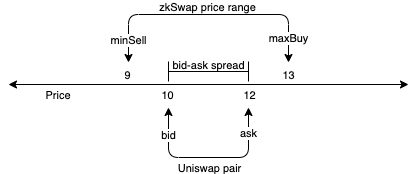
\includegraphics[totalheight=3cm]{diagrams/priceing.png}}
    \caption{Bid-ask spread and zkSwap price range}
    \label{fig:price}
\end{figure}

While this method ensures a 'worst-case' price for a trade, at the same time a maximum price is defined with it. Since we're matching buy and sell orders in one aggregation, there is no way around this. Once the aggregation is completed and verified on-chain, the new minSell and maxBuy prices are set, based on queried Uniswap prices, which are valid for the next aggregation batch.

% This price range is queried from the uniswap contract, and updated after each trade aggregation. When the net trade is executed, it is ensured that the price at least matches the worst-case price defined, or is lower. The aggregator can then pass the effective price on to the users. Once the trade aggregation is verified on-chain, it is ensured the effective price at least matches the stored worst-case price. Through this process, it is ensured the user is receiving a fair price. Ensuring the aggregator is claiming the actual effective price is an open problem and will be covered in S. XX
% A net trade will be executed, if the following condition is met:
% Lets say a Alice wants to sell 10 ZKS tokens on zkSwap. When creating the order, the form will display the minimal amount received, which in our case would be 90. The direction of the net trade doesn't matter. If the net trade is a sell, the trade will only execute if the price is \>\= 9, which fulfills the price range defined for the aggregation. If the net trade is a buy, Alice could receive up to 130 for her sell, depending on the actual price on Uniswap. If the price is higher, the trade will also not execute. 
% that is deemed acceptable for all trade orders, buy and sells. For this purpose, the zkSwap smart-contract stores a minSell and maxBuy price. The resulting range 
% predictable before the aggregation has started. 
% which can be a buy or a sell order. This trade needs to be executed, to cover all trade orders that are part of the aggregation. It is not possible to predict the direction of the `net trade', since orders of variable size and direction can be added at any moment.  
% The price between assets is constantly changing. At the same time, we're collecting trades in order to aggregate them. This results in a delay between an user sending a trade order and the actual trade execution, during which the price can change drastically. On top of that, a spread exists in the pricing of a trading pair. This means, that the current buy price doesn't equal the current sell price. 
% At the same time, we're aggregating buy and sell orders with each other, resulting in the net trade, which needs to be executed in order to cover all orders. It is not possible to predict the direction of the `net trade', since orders of variable size and direction can be added at any moment. Typically, a trade pair has a spread\footnote{The spread in a trading pair is the difference between current buy and sell prices}. This means the direction of a net trade can 
% single trade in either direction, that is needed to cover all aggregated trades. Predicting which direction the `net trade' will trade in is not possible. For this reason the zkSwap smart-contact stores a minSell and maxBuy price. It can be seen as a price range which is deemed acceptable for all orders part of an aggregation. When the `net trade' is executed on uniswap and the price has moved out of that range, the agregation is canceled. 
% his is an important mechasnism, because prices can change drastically while an aggragation is running or still collection orders. 
% price for buy and sell orders, which is used to calculate the trade order. 

\paragraph{Authorizing an Order}
Since this operation is running off-chain, we first need to verify the user is authorized to make the trade order. This can be achived by requesting a signature from the user, verifying it is in controll of the addresses private key. However, it must be remembered, that this signature must also be verifiable in our ZoKrates programm, which is unable to utilize the secp256k1 curve, used for signing Ethereum transaction, efficiently \cite{deml_2019}. For that reason the BN128 curve is used in combination with the EdDSA signature scheme, which can be more efficiently run in a ZoKrates program. The user signs the trade order and current balance root, ensuring two things. It proves that the user has access to the addresses private key, which authorizes the trade order. By signing the balance root, we make sure, that the signature can't by reused in a replay attack. For instance, the aggregator could decide to store these signatures secretly, and reuse them without the users consent if this was omitted. 

When the trade order is received, the aggregator first checks if the signature is valid and contains the current balances root, by querying it from the zkSync smart contract. As a next step, it is ensured, the users balance is able to cover the trade. The aggregator queries the merkle tree for the users balance, and checks if the trade can be covered by deposited funds. A last thing to consider is ensuring the correct price of a trade. The aggregator checks if the implied price of the trade matches the `worst-case' price stored in the zkSwap smart-contract. If all of these checks pass, the order is added to the trade pool, where it resides until the aggregation starts.  

\begin{figure}[h]
    \centerline{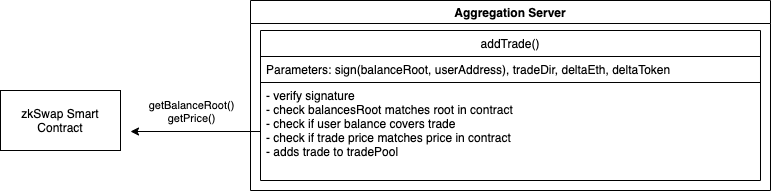
\includegraphics[totalheight=3cm]{diagrams/addTrade.png}}
    \caption{Pseudocode of addTrade()}
    \label{fig:addTrade}
\end{figure}

\paragraph{Running the Aggregation}
At some point the trade aggregation is started. This could be triggered by a set blocknumber, the number of trade orders that have been received or any other useful condition defined by the aggregator. When aggregation is started, the first step is to calculate the `net trade'. Since our system aggregates buy and sell orders, we can first offset those internally. By doing this, we're able to reduce the entire aggragation to one Uniswap trade, which saves gas. At the same time, we're saving on the 0.3\% liquidity provider fee, which is charged based on a trades volume. The net trade is the result of off-setting all trades in aggregation, which results one side to equal zero. This trade is now sent as an on-chain transaction to the `PairProxy` contract. The PairProxy contract is explained in detail in S. \ref{pairProxy}. 

The aggregator waits for the PairProxy smart-contract to emit the `TradeComplete' event, containing the amount of assets aquired in the Uniswap trade. The amount must at least imply the worth-case price, defined by the zkSwap smart-contract. In most situations, the implied price (effective price from here) will be better then the worst-case price. Based on the effective price, the users post-trade balances are calculated. Calculating the balances, poses a problem which arises by aggregating buy and sell orders in the same batch, which will be discussed in the limitations/open problems section. 

When the new balances have been created, the aggregator triggers the witness generation of the ZoKrates program. To execute the merkle inclusion proofs in the ZoKrates program the multi-leaf merkle path is generated and passed as an parameter, along with the old and new balances and the effective prices, paid in the trade step. This is described in detail in S. \ref{zokrates}. Once the witness has been generated, the proof generation is started, which results in the proof objects needed for the on-chain verification of the entire aggregation. To verify everything on-chain, and thereby updating balances of all all balances involved in the aggregation, the proof object is passed, along with the new balances, the old merkle root, the new merkle root, the effective net trade and the effective price and sent to the PairProxy smart-contract. At this point, the net-trade represents the funds that need to be exchanged by the PairProxy and the zkSwap smart-contract, to reimburse the aggregator for the funds spent in the Uniswap trade. 

\subsubsection{PairProxy Smart Contract} \label{pairProxy}
Before explaining the functionalities of this smart-contract, it is important to understand why it is required for the system to function. There are two reasons, a quirk in the way Ethereum handles return values, and the result of dealing with changing price data.
When performing a trade on Uniswap, a user is asked to define a slippage\footnote{Slippage is the difference of the expected and executed price of a trade} for the trade. Since network congestion and the current gas price influence when a transaction is executed, it's a neccecary mechansism for ensuring users can set a `worst-case' price. For this reason, when sending a transaction to the Uniswap trade function, the minAmountReceived parameter must be passed, which we provide by using our `worst-case` price, explained in a previous section. When calling the trade function, the actual amount received is returned as the functions return value. Since this amount might be larger then the amount passed as minAmountReceived, we need it to calculate the post-trade balances\footnote{The trade also throw an error, when the minAmoutReceived amount can't be fullfilled. In this case the aggregator cancels the aggregation}. 

However, a quirk in Ethereums way of handling return values makes this more difficult. A smart-contracts functions return value can only be accessed, when called by another smart-contract function. If calling a function as a normal transaction, as the aggregator does, instead of receiving the return value of the function, we receive the transaction recipe, which doesn't contain the return value. For this reason, we need the PairProxy smart-contract, which receives transanactions, forwards them to the respective smart-contract, emitting the return value as an event, which can be consumed by the transactor. 

The PairProxy smart-contract is used for forwarding transactions to the Uniswap or the zkSwap contracts. After the aggregator has calculated the `net trade', it calls the trade function in the PairProxy contract, passing the calculated trade parameters. The PairProxy contract now calls Uniswaps trade function, receiving funds and the amount as a return value. As it has access to the return value, it emits the `TradeComplete' event, containing the amount received in the trade. As it would be inefficient to send the funds back to the aggregator, they reside in the smart-contract. Since the aggregator is set as the owner of the contract, the funds are stored securly.

When verifying the aggregated trades in the zkSwap smart-contract, the transactions is forwarded by the PairProxy again. Since the funds previously traded still reside in the smart-contract, they are attached to the transaction when forwarded to the zkSwap smart-contract.


\subsubsection{ZoKrates Program} \label{zokrates}
The tasks and checks performed by the aggregator ensure that the trade aggregation is done correctly. It was verified a every trade order is authorized by the user, a users balance can cover the trade and that each order contained the correct worst-case price stored in the zkSwap smart-contract. However, this would require us to trust the aggregator, which is not the goal of this implementation and zk-rollups in general. For this reason, we rely on the properties of zkSNARK to make the correctness of the aggregations verifiable on the blockchain in a compressed form. \todo{Then general properties will described in background i guess} It is important to note, that the aggregator has computed all values needed for the trade aggregation. The ZoKrates program is only used to verify the correctness of the computed values. For efficiency we pass those computed values to the ZoKrates program, which will check them for correctness, defined in the program.

\paragraph{Merkle Multi-leaf Inclusion Proofs} 
In order to ensure the correctness of balance updates, we first need to verify the inclusion of the balances involed in the merkle tree. Doing this one by one is simple. Every leaf provides its merkle path which can be hashed with the leaf. If the merkle root matches the current merkle root, we can be assured the provided balance leaf is correct. At the same time, this enables us to reuse the merkle path for updating the balance leaf. We can simply change the balance leafs values after passing the inclusion proof, rehash with the merkle path, and the result is the correct root for the updated balance leaf. 

When dealing with multiple balance leafs, the inclusion proof can be done the same way. Every balance leaf provides its merkle path, the resulting hash should be the same for each leaf. Things become more difficult when updating the balance leafs. Updating the first leaf in the batch now invalidates the merkle path of all following leafs. This could be solved by sorting the leafs before hand, and generating each merkle path based on the changes of the previous leaf. At the same time, this results in the merkle path to be invalidated when proving the inclusion, so a seperate path for would be needed, which in turn undermines the validity of the proof. Another solution is needed. 

A multi-leaf inclusion proof ensures that the same merkle path can used for checking inclusion and updating the entire tree. Instead of generating a seperate merkle path for each leaf, we can construct the path in a way, that can be used with any number of leafs. We can now verify the inclusion of a balance and update these balances by hashing the tree twice in total, using the same merkle path for every leaf. This solves all problems described above. Since we now have a list of leafs, we need a way to decide if the next hash is computed with the next element of the merkle path or the next balance. For this reason we introduce proof flags. The proof flags are a boolean list, containing an element for each hashing operation needed to recreate the tree, ensuring we hash the correct values with each other. 

\begin{figure}[h]
    \centerline{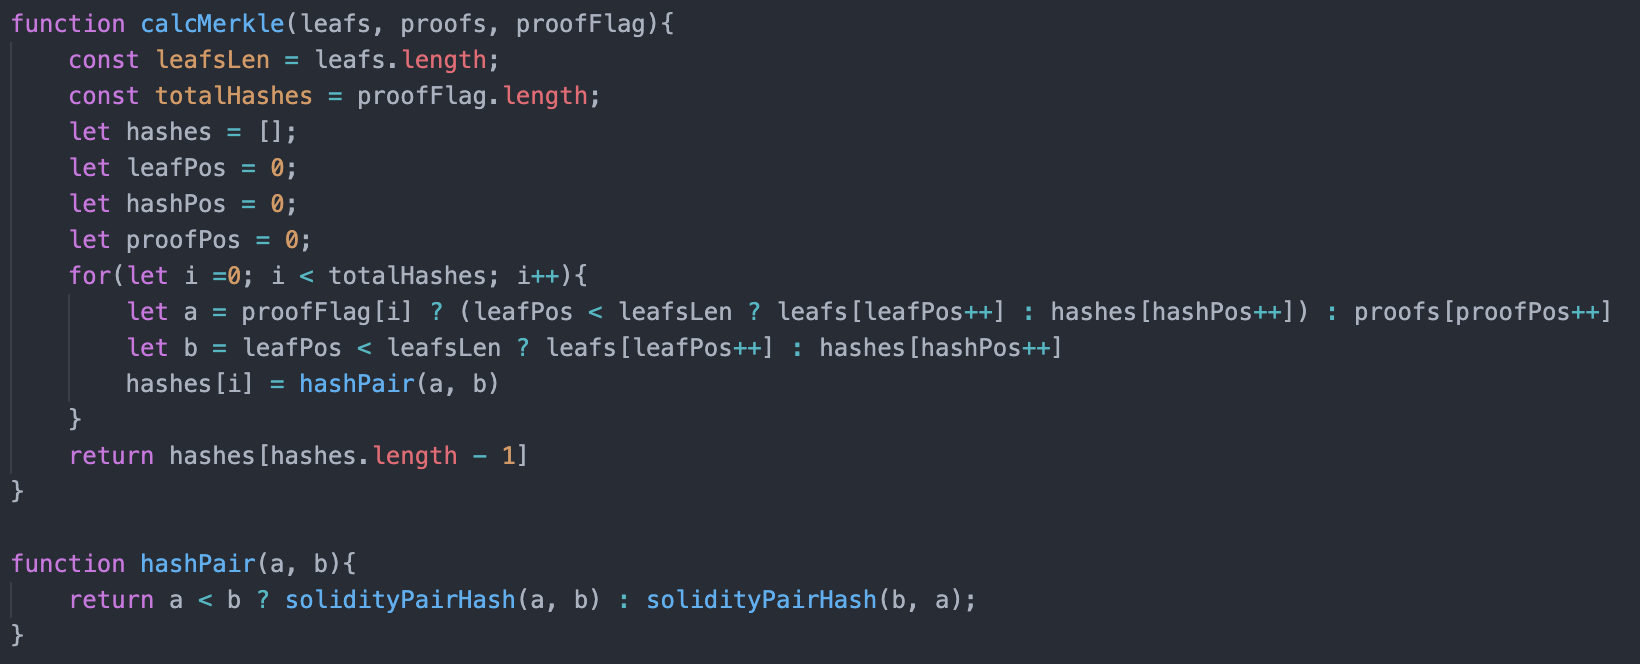
\includegraphics[totalheight=5cm]{diagrams/multi-leaf.png}}
    \caption{Multi-leaf Inclusion verification. TODO: Transform to algo notation}
    \label{fig:multiLeaf}
\end{figure}

The first check performed in the ZoKrates program, is the multi-leaf inclusion proof, shown in F. \ref{fig:multiLeaf}. We pass the old balances, merkle path and proof flags, receiving the computed merkle root as a result. If the merkle root equals the root that has been passed, we can be assured these balances are correct\footnote{The zkSwap contract ensures the root that was passed to the ZoKrates programm corresponds to the one stored in the contract}.

\paragraph{Checking Balance Updates and Signatures}
As the old balances of users have now been verified, the next step is to check if the state transistions, resulting in the new balances, are correct. The first thing to be check is the trade order and the corresponding signature. Depending on the trades direction, the amount paid for the trade is checked with the new balance. This ensures, the trade size has not been changed by the aggregator. If the signature can be verified, we are assured the order is authorized and the size correct. The price implied by the balance transistions also needs to be checked, making sure it matches the effective price reported by the aggregator\footnote{The correctness of this is checked in th zkSwap contract}. It is also checked if the nonce is incremented correctly. While checking balances, the net trade is calculated in the ZoKrates program, which is needed to check the on-chain flow of funds between the PairProxy and zkSwap smart-contracts at a later stage. 

\paragraph{Computing new Merkle Root}
As the correctness of balances and the state transitions have been proven, the next step is to compute the new merkle root. As mentioned above, we can do this by reusing the merkle path and proof flags, but passing the new balances as leafs this time. The resulting hash is the new merkle root, that will be stored in the zkSwap contract when the aggregation is verified on-chain. 

\paragraph{Reducing On-chain Verification Costs}
We have now successfully verified the new balances, and we could use these values to generate the proof, which will then be used to verify everything on-chain. When verifying the ZoKrates program on-chain, each output of the program is part of the proof object, adding an iteration to the proving logic. The amount of outputs the ZoKrates program has, influences the verifications costs. We can reduce this cost by returning a hash of the resulting data, thereby reducing the amount of outputs. Since the aggregator computed the balances in the first place, and the ZoKrates program only verified it, it can pass that data as part of the verify transaction, but excluded from the ZoKrates proof object. By hashing the data in the zkSwap smart contract, we can ensure that data correctness by comparing it to the hash that is part of the proof object. As a result, the ZoKrates program only returns this hash as an output value. 
\todo{Explain assumtions that can be made from proof in background, hashing as algo blaaa}

\begin{figure}[h]
    \centerline{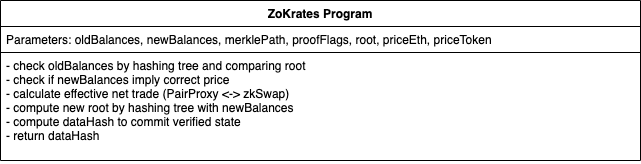
\includegraphics[totalheight=3cm]{diagrams/zokrates.png}}
    \caption{ZoKrates program checks}
    \label{fig:zokrates}
\end{figure}

\subsubsection{Client Frontend}
The frontend allows the user to interact with the system, calling the functions, while providing neccecary data is the background. The frontend also listens for `BalanceUpdate' events and keeps the merkle tree in sync locally. This allows the client to access the merkle tree in order to provide the merkle path for a transaction for example, without relying on an external system to provide this data. In its current design, the frontend could be hosted as a static file in IPFS \cite{benet2014ipfs}, not relying on any server to facilitate withdraws of user funds, which closely follows Ethereums unstopable applications ethos. Running this with a large merkle tree becomes unfeasible quickly though, so a hybrid approach can be envisioned. A server is used to provide the user with requested data from the merkle tree. If the server is offline or provides incorrect data, the client can sync merkle tree itself. While this would put computational strain on the client, it ensures that a user is always able to withdraw funds, no matter what entities are offline or have turned malicious. 

\paragraph{Deposits and Withdraws}
In order to deposit and withdraw funds, the users needs to specify a number of parameters, that are needed to execute the transaction. First of all the merkle path is needed, which the client can generate by querying its local instance of the merkle tree. The balance object can also be provided by the merkle tree. A form in the frontend is used to define the amounts wishing to be deposited/withdrawn, which will gather the neccecary parameters and add them to a Ethereum transaction. Metamask or any other browser compatible wallet will open, summarizing the transaction, which a user can now sign, bringing it on chain. Once the `BalanceUpdate' event is fired, the frontend will update the balance in its merkle tree.

\paragraph{Adding a Trade}
When adding a trade a user defines the direction of the trade and the amount wishing to be traded. The trade form will display a minimal amount received, which is calculated based on the worst-case price for either trade direction. Since this is an off-chain transaction, when sending the order a user is asked to sign the order and the current balance root with its addresses private key, explained in detail in S. \ref{aggregator}\ref{zokrates}. The order is now sent to the aggregator as an HTTP request. 

\paragraph{Displaying Account Data}
The frontend also displays basic account data, which makes usage of the system easier. This includes the accounts current balances, as well as the address. Redux is used in the background to keep the data in sync.

\subsection{Limitiations of Current Implementation}
The final implementation of this work does not include all attributes mentioned in the previous sections. 

\paragraph{Signatures}
As described in S. \ref{aggregation_server}, the authorization of an order entirely relies on a user signing the trade order and merkle root. This signature needs to be checked in a ZoKrates program, which limits us to use the EdDSA scheme, in combination with the BN128 curve. However Metamask, a browser compatible Ethereum wallet, does not support this. Since the private key is stored in Metamask, there are no theoretical limitiations in adding the curve in signature scheme, it simply hasn't been done yet. The outlook section will also look at alternative solutions\todo{BLS aggregate signatures}. For this reason, the signature checks are omitted in the prototype, their computational cost is included in the results section though.

\paragraph{Updating Balances According to Effective Price}
After the aggregator has executed the net trade on Uniswap, the new balances are calculated based on the worst-case price instead of the effective price the aggregator has paid. Currently, there is no mechanism in place that can ensures this. The aggregator could always claim the worst possible price has been paid (depending on net trade direction), while keeping the difference for itself. This will be addressed in the open problems section.

\paragraph{Arbitrary Combinations of Merkle Tree Leafs}
In its current form, each aggregation must contain three trades, and the involved balances must be neighbors in the merkle tree. When creating the Merkle multi-leaf inclusion proofs, the positions of the leafs in the tree influences the number of hashes in the merkle path. Each hash value in the merkle path needs to be hashed once as part of the inclusion proof, so a longer merkle path results in a higher number of hashes being computed. Two leafs that are a pair in the tree, contain the same number of hashes in the merkle path as a single leaf does\footnote{Actually, the merkle path is one element smaller when generated for two pair leafs, as the neighboring leafs hash has moved from the merkle path, to the leafs list.}. If the leafs are at the opposite half of the tree, the number of hashes in the merkle path almost doubles. This makes implementation in ZoKrates more complicated, as it can not deal with arbitrary length data. This can be solved by compiling a number of different versions of the program, all accepting different merkle path lengths, which will be covered in the limitations section.


% This poses a problem, what use is a cheap data storage, if it can be queried from a client 


% The different functions that can be used to update balances will be described at a later point, 

% To achive this, we store balances in a merkle tree in layer-2, each balance stored as a seperate leaf. Merkle trees are a suitable data structure, as the root represents the entire tree state in a highly compressed form, while proving a leafs inclusion in the tree can be done with O(log n). This is ideal for our use-case. We can cheaply commit the merkle trees state to our smart-contract by storing the root, while verifying inclusion of a leaf is very efficient. The different functions that are can be used to update balances will be discussed at a later point, it is important to understand the core technique used for storing balances beforehand.
% The zkSync smart-contract is the only entity in the system that is able to update balances. Since we don't want to rely on external data availability, we need to store state on-chain, but as cheaply as possible. We can do this by emitting an event, thereby writing data to the event log. While the event log can't be accessed from a smart-contracts runtime, it is significantly cheaper then storing data in a smart-contracts storage. 
% a client can query the event log and pass the data as a parameter


% To deposit funds, a user need to provide a valid merkle path to its current balance and the current balance object. The user calls the deposit function, passing the merkle path and balance object as a parameter and adds the funds wishing to be deposited to the transaction. 

% First we check if the balance is included in the tree. To do this, we first hash the balance object with the sha256 algorithm. The balance object contains the following fields: ethBalance, tokenBalance, nonce and address. When hashing the balance object, we extract the users address from the transaction. This ensures that the user is in control of the addresses private key which suffices as security check. Since the contract stores the merkle root, we can now hash the path and balance, checking if we can recreate the root. If the roots match, the trader is permitted to update its balance in the tree. We now update the balance object by adding the deposited amount to the corresponding field, increment the nonce, hash the updated balance object, and rehash the entire tree with the the new balance object. The resulting merkle root is set in the contract, which commits the updated state. 

% However, we still need to store the balances somewhere. As we don't want to rely on external data availability, while keeping storage costs as low as possible, we emit the new balance as an event. Writing data to the event log is a lot cheaper, compared to storage as a variable in a smart-contract. While the event log can't be accessed from a smart-contracts runtime, a client can query the event log and pass the data as a parameter. As the merkle trees state is committed in the contract with the merkle root, correctness can always be proven. 

% Withdrawing funds follows the same logic as deposits. Instead adding funds to the withdraw function, the user passes the amount to withdraw as a parameter. The merkle tree is rehashed, checking if the root is correct, it is ensured the withdrawAmount <= balance, the balance and nonce are updated, creating the new root. We emit the new balance and send the funds to the user. 

% Deposits and withdraws are complete on-chain operations by design. All data needed to withdraw funds are public, except for the private key. This ensures funds can always be withdrawn, as long as the user controlls its private key.

% A trader can deposit funds, by providing a valid merkle path to its current balance as parameters to the zkSwap contract. 




% A trader looking to use the system first needs to deposit funds into the zkSync smart-contract.


% If successful, the deposited amount will be represented as a balance in layer-2. In layer-2, balance objects are stored in a merkle tree, while the root of that tree resides in the zkSync smart-contract. 

% and the amount represented as a balance in layer-2. 

% Since the goal is to store them in layer-2, while remaining free of any external data availability, a somewhat hybrid approach is needed. A trader always must be able to withdraw balance, no matter how many entities are offline. 

\end{document}